\chapter{Evaluation}

This chapter presents an evaluation of SecArchUnit in terms of performance and usability when compared to static analysis tools used in industry. The results are discussed and related to the research questions. Finally, a discussion is held regarding the validity threats of the evaluation.

\section{Results}
This section presents the results of the evaluation in two steps: first the evaluation relating to how effectively SecArchUnit and similar tools validate the constraints, and then an evaluation of differences between the tools in terms of their usability.

\subsection{Performance}\label{sec:performance_results}
The performance evaluation aims to evaluate how well SecArchUnit can validate the 7 constraints and compare this to the performance of industrial-grade tools SonarQube and PMD. Due to the fact that not all constraints could be expressed in the tools used for comparison, the evaluation was divided into two stages: a comparison of all tools using the first 5 constraints, and a review of the performance of SecArchUnit regarding constraints 6 and 7.

For both stages, the tools were evaluated according to the performance metrics. The true positives (TP) refer to violations of constraints that are reported by the tool and coincide with the ground truth. False positives (FP) are violations reported by the tool that are not included in the ground truth. False negatives (FN) are violations that exist in the ground truth but do not get reported by the tool. 

\newcolumntype{g}{>{\columncolor{RowColor}}c}
\newcolumntype{x}{>{\columncolor{RowColor}}l}
\begin{table}[h]
\begin{center}
\begin{tabular}{lxggggg}
\rowcolor{white}
\textbf{Project}           & \textbf{Tool}    & \textbf{TP} & \textbf{FP} & \textbf{FN} & \textbf{Precision} & \textbf{Recall} \\
\hline
\rowcolor{white}
\multirow[t]{3}{*}{ATMsim}    & SecArchUnit      & 19          & 1           & 0           & 1               & 0.95            \\
                           & SonarQube Plugin & 19          & 1           & 0           & 1               & 0.95            \\
                           \rowcolor{white}
                           & PMD Plugin       & 15          & 1           & 4           & 0.94               & 0.79            \\
\hline
\rowcolor{white}
\multirow[t]{3}{*}{JPetStore} & SecArchUnit      & 51          & 0           & 0           & 1                  & 1               \\
                           & SonarQube Plugin & 51          & 0           & 0           & 1                  & 1               \\
                           \rowcolor{white}
                           & PMD Plugin       & 47          & 0           & 4           & 1                  & 0.92            \\
\hline
\rowcolor{white}
\multirow[t]{3}{*}{ITrust}    & SecArchUnit      & 216         & 3           & 0           & 0.97               & 1               \\
                           & SonarQube Plugin & 216         & 0           & 0           & 1                  & 1               \\
                           \rowcolor{white}
                           & PMD Plugin       & 216         & 0           & 0           & 1                  & 1 \\
\hline
\end{tabular}
\end{center}
\caption{Results from validating constraints 1-5 using SecArchUnit, SonarQube and PMD.}
\label{tab:results_comparison}
\end{table}

As seen from Table~\ref{tab:results_comparison}, all three tools performed well in regards to both precision and recall. Since each tool's rules were evaluated against the same collection of classes, the set of detected violations is the same for all tools. Overall, very few false positives and false negatives were found, making up for less than 5\% of the total amount of reported violations when counting unique cases across all tools and systems. 

As depicted in Figure~\ref{bar:frequency_violation_comparison}, constraint 1 accounts for the majority of all violations found in the three projects. Violations of constraint 5, on the other hand, were not found in any project; thus, we can not draw any conclusions regarding the tools' reliability of detecting that particular violation. Additionally, violations of constraints 2 and 3 were sparse and not consequently found in all systems.

\begin{figure}
\centering
\captionsetup{justification=centering}

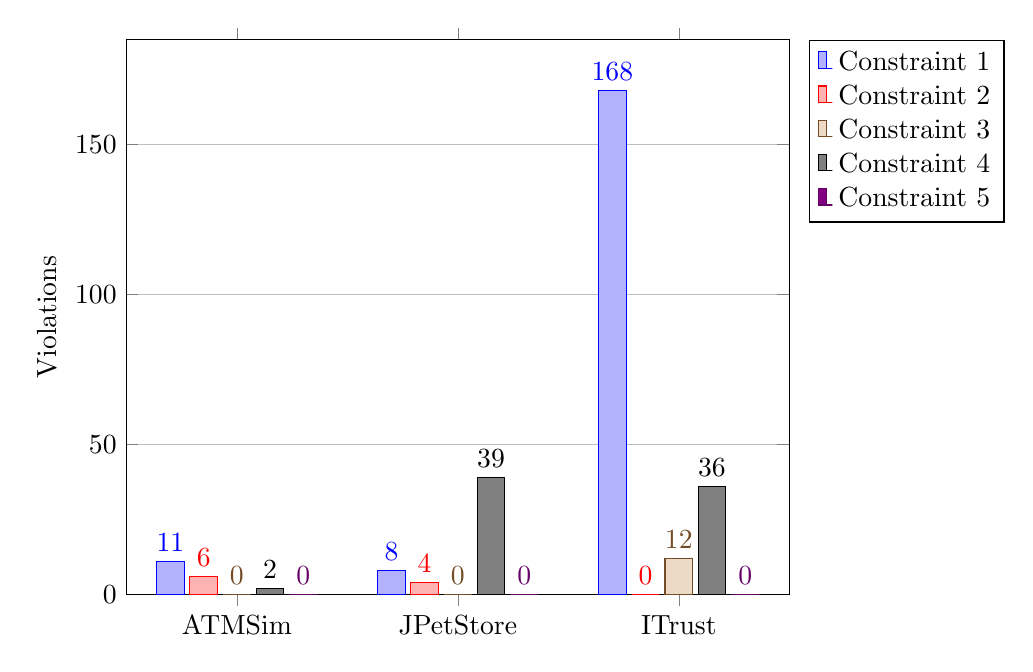
\begin{tikzpicture}
\begin{axis}[
    width=10cm,
    ybar,
    ymin = 0,
    ymajorgrids = true,
    enlarge x limits=0.25,
    xbar legend,
    legend pos=outer north east,
    ylabel={Violations},
    symbolic x coords={ATMSim,JPetStore,ITrust},
    %xlabel={System},
    xtick=data,
    nodes near coords,
    nodes near coords align={vertical},
    ]
%C1
\addplot coordinates {(ATMSim,11) (JPetStore,8) (ITrust,168)};
%C2
\addplot coordinates {(ATMSim,6) (JPetStore,4) (ITrust,0)};
%C3
\addplot coordinates {(ATMSim,0) (JPetStore,0) (ITrust,12)};
%C3
\addplot coordinates {(ATMSim,2) (JPetStore,39) (ITrust,36)};
%C3
\addplot coordinates {(ATMSim,0) (JPetStore,0) (ITrust,0)};
\legend{Constraint 1,Constraint 2,Constraint 3, Constraint 4, Constraint 5}
\end{axis}
\end{tikzpicture}

\caption{The constraint violations found in the ground truth of each system.}
\label{bar:frequency_violation_comparison}
\end{figure}

In the second stage, constraints 6-7 were applied to the test systems and validated solely using SecArchUnit. The performance metrics resulting from this evaluation are presented in Table~\ref{tab:tool_extension}. In iTrust, SecArchUnit reliably detected violations of both constraints, resulting in high precision and recall. In contrast, JPetStore had no violations that could be assessed, whereas ATM Simulation failed to report one of its two violations, and additionally reported two false positives, resulting in poor precision and recall.

\begin{table}
\begin{center}
\begin{tabular}{lccccc}
\hline
\textbf{Constraint} & \textbf{TP} & \textbf{FP} & \textbf{FN} & \textbf{Precision} & \textbf{Recall} \\
\hline
6 & 24 & 0 & 0 & 1 & 1\\
\rowcolor{RowColor}
7 & 37 & 0 & 0 & 1 & 1\\
\hline
\end{tabular}
\end{center}
\caption{Results from validating the extension-based constraints on iTrust.}
\label{tab:tool_extension}
\end{table}

Looking at the distribution of constraint violations for constraint 6 and 7, found in Figure~\ref{bar:frequency_violation_extension}, we can see that in iTrust, both constraints had enough violations to allow for an evaluation, whereas in ATM Simulation and JPetStore, there were very few violations. This is attributed in part to the differences in size between these two projects and iTrust, and in part to the fact that JPetStore had no logging functionality.

\begin{figure}
\centering
\captionsetup{justification=centering}

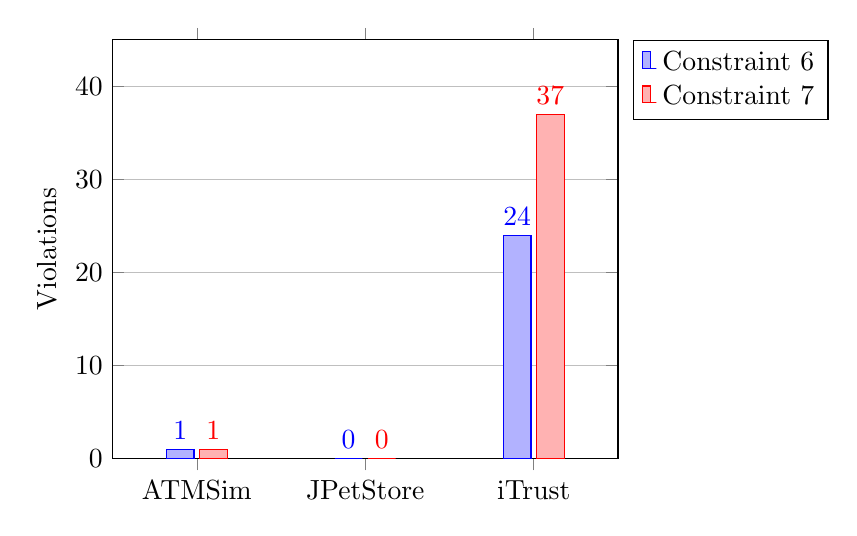
\begin{tikzpicture}
\begin{axis}[
    width=8cm,
    ybar,
    ymin = 0,
    ymax = 45,
    ymajorgrids = true,
    enlarge x limits=0.25,
    xbar legend,
    legend pos=outer north east,
    ylabel={Violations},
    symbolic x coords={ATMSim,JPetStore,iTrust},
    %xlabel={System},
    xtick=data,
    nodes near coords,
    nodes near coords align={vertical},
    ]
%C6
\addplot coordinates {(ATMSim,1) (JPetStore,0) (iTrust,24)};
%C7
\addplot coordinates {(ATMSim,1) (JPetStore,0) (iTrust,37)};

\legend{Constraint 6,Constraint 7}
\end{axis}
\end{tikzpicture}

\caption
    [Violations of constraint 6 and 7 asserted in the ground truth]
    {The violations of constraint 6 and 7 asserted in the ground truth.}
\label{bar:frequency_violation_extension}
\end{figure}

Finally, the performance of SecArchUnit for each constraint across all systems can be seen in Table~\ref{tab:secarchUnit_constraint}. We can infer from data that SecArchUnit reliably detects violations of all constraints except for constraint 5 as it was not present in any of the systems. 

\begin{table}[h]
\captionsetup{justification=centering}
\caption
    [Performance of SecArchUnit for each constraint across all test systems]
    {The performance of SecArchUnit for each constraint across all test systems.}
\begin{center}
\begin{tabular}{lccccc}
                    \textbf{Constraint}  & \textbf{TP} & \textbf{FP} & \textbf{FN} & \textbf{Precision} & \textbf{Recall} \\
\hline
1 & 167         & 3           & 0           & 0.98      & 1          \\
\rowcolor{RowColor}
2 & 10          & 0           & 0           & 1      & 1          \\
3 & 12          & 1           & 0           & 0.92      & 1          \\
\rowcolor{RowColor}
4 & 87          & 0           & 0           & 1      & 1          \\
5 & 0           & 0           & 0           & -      & -         \\
\rowcolor{RowColor}
6 & 24 & 0 & 0 & 1 & 1 \\
7 & 37 & 0 & 0 & 1 & 1 \\
\hline
\textbf{Mean}         &             &             &             & 0.98      & 1         
\end{tabular}
\end{center}

\label{tab:secarchUnit_constraint}
\end{table}

\subsection{Usability}
The tools were additionally evaluated in terms of their usability. Firstly, the effort required to express the constraints in the different tools was considered. This effort was quantified as the amount of time spent implementing the rule pertaining to each constraint. These results can be seen in Figure~\ref{fig:Design_time}. From the figure, and the fact that the constraints were implemented sequentially, we can infer that the time required to implement new constraints decreases following increased knowledge of the tools. As constraint 4 included additional functionality, in the form of inspecting annotations, an increase in time can be seen between constraint 3 and 4. For both SecArchUnit and SonarQube, the time to implement is significantly reduced when later implementing constraint 5. PMD, on the other hand, does not see the same decrease. The absence of decreased time was attributed to the fact that there was additional work involved with extracting and checking annotations in PMD, which we distributed equally between the two constraints. Excluding the first 2 constraints, SecArchUnit required a total of 10 hours to implement the constraints, whereas SonarQube and PMD required 16 and 21 hours respectively. 

\definecolor{lightblue}{RGB}{102, 178, 255}

\begin{figure}
    \centering
    \captionsetup{justification=centering}
    \begin{tikzpicture}
    \begin{axis}[
        width = 11cm,
        ybar,
        ymin=0,
        ymajorgrids=true,
        enlarge x limits=0.20,
        xbar legend,
        legend pos=outer north east,
        ylabel={Time to implement (hours)},
        symbolic x coords={SecArchUnit,SonarQube,PMD},
        xtick=data,
        nodes near coords,
        ]
    % C1
    \addplot[black, postaction={pattern=north east lines}] coordinates {(SecArchUnit,6) (SonarQube,8) (PMD,10)};
    % C2
    \addplot[black, postaction={pattern=north east lines}] coordinates {(SecArchUnit,5) (SonarQube,9) (PMD,9)};
    % C3
    \addplot[blue, fill=blue!30!white] coordinates {(SecArchUnit,3) (SonarQube,5) (PMD,6)};
    % C4
    \addplot[red, fill=red!30!white] coordinates {(SecArchUnit,5) (SonarQube,7) (PMD,8)};
    % C5
    \addplot[brown!60!black, fill=brown!30!white] coordinates {(SecArchUnit,2) (SonarQube,4) (PMD,7)};
    \legend{Constraint 1,Constraint 2,Constraint 3, Constraint 4, Constraint 5}
    \end{axis}
    \end{tikzpicture}
    \caption
        [Time to implement each constraint]
        {Time to implement each constraint.}
    \label{fig:Design_time}
\end{figure}



Secondly, the time required to validate the constraints, i.e. the running time of each tool, was considered. The tools were executed three times on each system to improve the accuracy of the measurement. These results are presented in Table~\ref{tab:benchmark}. SecArchUnit and PMD perform similarly on the two smaller systems, with both finishing in approximately 1 second. In contrast, the time required for SonarQube to finish is increased by a factor of ten. When validating iTrust, there is an apparent disparity between SecArchUnit, which completes its validation in 2 seconds, and PMD and SonarQube, which complete their validation in 7 and 39 seconds, respectively.

%\newcolumntype{g}{>{\columncolor{RowColor}}c}
%\newcolumntype{x}{>{\columncolor{RowColor}}l}
\begin{table}
\captionsetup{justification=centering}
\caption
    [Run time benchmarks]
    {Run time benchmarks from validating the constraints in each tool and system, measured in 3 consecutive runs.}
\begin{center}
\begin{tabular}{lxggggg}
\rowcolor{white}
\textbf{Project} & \textbf{Tool} & \textbf{Mean time (s)} & \textbf{sd} \\
\hline
\rowcolor{white}
\multirow[t]{3}{*}{ATMSim}
        & SecArchUnit & 0.957 & 0.072 \\
        & PMD Plugin & 1.3 & 0.078 \\
        \rowcolor{white}
        & SonarQube Plugin & 13.7 & 1.7 \\
\hline
\rowcolor{white}
\multirow[t]{3}{*}{JPetStore}
        & SecArchUnit & 0.837 & 0.035 \\
        & PMD Plugin & 1.46 & 0.21 \\
        \rowcolor{white}
        & SonarQube Plugin & 12.4 & 0.50 \\
\hline
\rowcolor{white}
\multirow[t]{3}{*}{ITrust}
        & SecArchUnit & 2.24 & 0.12 \\
        & PMD Plugin & 7.37 & 0.23 \\
        \rowcolor{white}
        & SonarQube Plugin & 39.4 & 3.25 \\
\hline
\end{tabular}
\end{center}
\label{tab:benchmark}
\end{table}



\section{Discussion of performance results}

Both in regards to precision, as well as recall, the tools performed equally. However, the causes of failure differed noticeably in cases where the results of the tools varied. The examples are described below:

\begin{itemize}
    \item In ATM Simulation, the same false positive occurred in all three tools. This was in relation to constraint 3, where a subclass of the sending point contained a method call to the sender. Additionally, PMD had 4 false negatives which occurred because it was unable to determine the classes that these method calls targeted.
    \item In JPetStore, PMD reported 4 false negatives, again because it was unable to determine the target class of these method calls.
    \item In iTrust, a security service contained both an inner interface and an inner static class whose methods did not perform any security events. In both PMD and SonarQube, these methods were determined to be declared in the inner class by traversing the AST from the method to its first parent class or interface declaration. In comparison, SecArchUnit considers the members of the inner class to be declared in both the inner and outer class. This improperly marks the inner methods as violating the constraint, resulting in 3 false positives in SecArchUnit.
\end{itemize}

As shown in Figure~\ref{bar:frequency_violation_comparison}, the tools were evaluated using imbalanced data. Constraint 1 accounted for a majority of all violations found throughout all three systems, while no system violated constraint 5. Additionally, iTrust was the only system to contain a violation of constraint 3. 

\textbf{Extension constraints.}
In ATM Simulation, the tool performed poorly when validating constraint 7. The false negative resulted from the fact that an object, which owned a secret field, was passed to the logger and converted to a string representation that exposed the secret \textit{inside} the logger class. Therefore, the hint to the secret field was not included in the arguments of the call to the logger and the constraint subsequently failed to catch the violation. In addition, SecArchUnit reported two false positives which were found after three recursion steps on the argument hints (access to method, which accesses method, which accesses getter method of the secret field). While the concerned method did indeed access the secret fields, neither of their values flowed into the return value of the method. Therefore, it is suspected that stack hints are improperly handled for some instructions during the analysis of the system.

The system, iTrust, initially contained no violations of constraint 7. Therefore, violations were injected by systematically marking all identifier fields (e.g. \texttt{patientId}, \texttt{personnelId}) in the model and base-action packages as secrets. We chose to mark these identifiers because they were commonly sent to the logger as a way to describe the patient or personnel involved in a transaction. Hence, the 37 violations of constraint 7 in iTrust, as seen in Table~\ref{tab:tool_extension}, are artificially injected.

Moreover, iTrust is built with a mix of Java and Java Server Pages (JSP) files whereas ArchUnit can only analyze plain Java. The classes in the action package, from which the logger is called, are all instantiated in the JSP files outside the view of our analysis. As such, the types of information flow that are analyzed and included in the ground truth are rather rudimentary. Out of the 37 violations of constraint 7, 1 was found without recursion (direct access to secret field) and the remaining 36 were found using a single recursion step (access to getter method of a secret field).
% This is bad - we could just as well put the secret annotation on the getter and enforce the same constraint in SonarQube/PMD

%\todo{Discuss examples of things that the tools won't catch}
% different levels of assets, i.e some fields are more sensitive than others



\section{Discussion of qualitative differences}
While SecArchUnit, SonarQube and PMD are all static analysis tools that support evaluation of custom rules, they differ considerably in how their rules are defined and evaluated.

SecArchUnit builds an architectural representation of the entirety of the analyzed system, which is available during the evaluation of the rules. As shown throughout Chapter~\ref{ch:enforcing_constraints}, rules have access to information about both incoming and outgoing accesses to all members, within and between classes, making it convenient to specify architectural constraints at an appropriate level of abstraction.

Regarding SonarQube and PMD, both of these tools evaluate rules by traversing an Abstract Syntax Tree (AST) that describes the source code of the system. While this allows the tools to enforce low-level code constraints by inspecting, for example, if-statements, try-catch blocks and the order of statements within a code unit, they do not lend themselves to specifying security architectural constraints. The implementations of constraint 1 in SecArchUnit and SonarQube can be seen in Listing~\ref{lst:secarchunit_1_excerpt} and Listing~\ref{lst:sq_1_excerpt}, respectively. The rule in SecArchUnit is defined in 4 lines, whereas the equivalent rule in SonarQube requires approximately 30 lines of code and multiple traversals of the AST to extract the information relevant to the constraint. Admittedly, the rule in SecArchUnit makes use of a custom condition which is defined in another 6 lines of code, but the difference is still considerable.

\begin{lstlisting}[caption={Constraint 1 in SecArchUnit.}, captionpos=b, label=lst:secarchunit_1_excerpt, numbers=left, showstringspaces=false]
return methods()
    .that().haveModifier(JavaModifier.PUBLIC)
    .and().areDeclaredInClassesThat(securityServicesDescriptor)
    .should(callMethod(declaredIn(logger)));
\end{lstlisting}

\begin{lstlisting}[caption={Constraint 1 in SonarQube. The definition of the entire class can be seen in Appendix~\ref{lst:sq_1}.}, captionpos=b, label=lst:sq_1_excerpt, numbers=left, showstringspaces=false]
String methodEnclosingClass =
  method.symbol().enclosingClass().name().toLowerCase();
if (!SECURITY_CLASSES.contains(methodEnclosingClass)) {
  return;
}

boolean isPublicMethod = false;
for (ModifierKeywordTree keywordTree : 
    method.modifiers().modifiers()) {
  if (keywordTree.modifier() == Modifier.PUBLIC) {
    isPublicMethod = true;
    break;
  }
}

if (!isPublicMethod) {
  return;
}

boolean containsCallToLogger = false;
ControlFlowGraph cfg = method.cfg();

for (ControlFlowGraph.Block block : cfg.blocks()) {
  for (Tree blockTree : block.elements()) {
    if (blockTree.is(Tree.Kind.METHOD_INVOCATION)) {
      MethodInvocationTree mit = (MethodInvocationTree) blockTree;
      if (loggerMethods.matches(mit)) {
        containsCallToLogger = true;
      }
    }
  }
}

if (!containsCallToLogger) {
  reportIssue(...);
}
\end{lstlisting}

In SonarQube and PMD, the root node of the AST is the Java class currently being analyzed. As a consequence, a rule can only inspect one class at a time; it can audit outgoing accesses from the current class, but it does not know anything about incoming accesses from other classes. In a constraint where incoming accesses to a specific class need to be restricted, these tools instead inspect all classes one by one and look for outgoing accesses to the concerned class.
This likely contributes to the inefficient validation of the constraints, as shown in the benchmarks, due to each rule traversing the AST of all classes in the system. In contrast, SecArchUnit uses the predicate to select only the elements relevant to the constraint, on which the condition is subsequently applied.

%\todo{Much like query optimization/indexing, in ArchUnit the relevant accesses are selected directly and then have a condition applied to them. The other tools go through all classes, once for every rule, which is less efficient and is reflected in the benchmarks}

%\begin{minipage}{\textwidth}
%\begin{lstlisting}[caption={Excerpt of constraint 3 in SonarQube, simplified using pseudo %code. See full rule definition in Appendix~\ref{apx:sonarqube} and the related PMD rule in %Appendix~\ref{apx:pmd}.}, captionpos=b, label=lst:sonarqube_excerpt, numbers=left, %showstringspaces=false]
%public void visitNode(MethodInvocation node) {
%    if (target method is declared in a sender) {
%        // Get class in which method invocation takes place
%        ClassTree classTree = node.parent() until type is ClassTree
%
%        if (classTree is not the sending point) {
%            reportIssue(...);
%        }
%    }
%}
%\end{lstlisting}
%\end{minipage}

In addition, these tools cannot enforce constraints where both incoming and outgoing accesses need to be inspected in unison. An example of this is constraint 4, where the constraint allows user input to be validated either by calling a validator or by only being called by validators. The rules in SonarQube and PMD can only look for outgoing calls to validators, not taking incoming accesses into account, and therefore risk reporting false positives. However, no such case was found in the evaluation.

When inspecting a method invocation node in the AST, SonarQube exposes information about the target method, including its signature, annotations, and information about the class in which it is declared. In PMD, however, the node that corresponds to method invocations only contains information about the return type of the method. In order to resolve the target class of a method invocation, we examined the immediately preceding expression. If the expression had a return type, this was assumed to be the target owner. Otherwise, the expression was further examined for references to local variables and fields, the declarations of which contained the necessary type information. This lack of type information not only made the constraints complicated to express, but it also resulted in an unreliable resolution of method targets, as reflected in the number of false negatives reported by the tool.

Moreover, PMD contains no information about the annotations that are present on the target method. As a workaround, a separate rule was created which visited all class and method declarations, dumping their annotations into a text file. This text file was then fed into the rules related to constraints 4 and 5.

To summarize, while it is possible for SonarQube and PMD to enforce some security architectural constraints, these rules are not expressed at the proper level of abstraction. This was made especially apparent in PMD, where several workarounds had to be devised in order to express the constraints.



\section{Answering research questions}
% RQ1: What architectural security constraints can be validated using the tool?
To answer the research question regarding which architectural security constraints can be validated using SecArchUnit (\textbf{RQ1}), the evaluation has shown that SecArchUnit can validate constraints 1-4, which relate to the security goals of confidentiality, integrity and accountability. Its performance, in terms of precision and recall, is comparable to tools used in the industry. As the evaluation found no violation of constraint 5, it remains unclear whether the tool can validate constraints related to the security goal of availability.

% RQ2: What modifications can be made to the tool in order to facilitate the validation of additional constraints?
To answer the research question regarding what modifications can be made to ArchUnit (\textbf{RQ2}), the evaluation suggests that the tool can be extended with an analysis of information flow, and that this can be leveraged to validate additional constraints relating to the security goal of confidentiality.



\section{Threats to validity}
This section presents the validity threats of the thesis. 

\subsection{Construct validity}
The primary threat to construct validity is whether the constraints considered in the study increases the security of a system. While we do not consider the enforcement of our constraints to provide a holistic approach to security, the relevance of providing a more secure system has been asserted by gathering established security measures.

\subsection{Internal validity}
In the absence of any preexisting ground truth, the threat of misinterpreting the architectural design of a system, and consequently, establishing an invalid ground truth is inherent. We reduced the threat of misinterpretation by having each author independently establish a ground truth, later comparing the results and carefully discussing the differences. Additionally, in cases where both of us were uncertain, our supervisors were consulted for further knowledge.


For our seventh constraint, \say{secrets must not be sent to a logger}, we found no violations as the developers of iTrust had ensured that the logger only received the appropriate information. To still be able to test the reliability of the extensions made to ArchUnit, we used data that was seen to be sent to the logger, although the data was non-sensitive. However, the functionality of SecArchUnit to support information flow constraints was still tested. 

As the constraints were implemented sequentially, the time required to implement each constraint in a tool is affected by a carry-over effect as we learn how to use the tool. Similarly, our knowledge of SecArchUnit, compared to the tools used for comparison, was greater, resulting in a biased result. The ramifications of both are minimized by excluding the first two constraints as a learning experience, and then considering the total time required to implement the remaining constraints.
% researcher bias?

\subsection{External validity}

We formed the constraints used in the study to be generally applicable and not dependent on any specific domain or framework. Additionally, the reference to previously established security patterns, weaknesses, or constraints should provide some assurance of the validity of the constraint to projects other than those included in the study. However, as no previous study has applied them to a broad set of projects, we cannot draw any conclusion on the general validity. 

Our choice of sample systems used in the evaluation represents another threat to external validity. We weighted several factors when deciding on which projects to use, such as the availability of architectural documentation, the size of the system, and whether they had been used in previous literature. Many open-source projects were discarded based on the fact that they did not provide any documentation for which we could establish the ground truth. Naturally, the size of a system profoundly affected the time needed for the architectural analysis, further reducing the set of systems that we could include. Thus, we tried to strike a balance between including project large enough to provide a realistic context, while at the same time being sufficiently small to allow for a rigorous analysis. We believe that while all three sample systems had initially been developed in the context of teaching, their implementation represents a realistic system. Additionally, the size of iTrust is large enough to warrant further validity.

